% Standalone copy of the latency chart in overview.tex (same data).
% Build: pdflatex latency_chart.tex, then convert the PDF to PNG.
\documentclass[border=10pt]{standalone}
\usepackage[T1]{fontenc}
\usepackage{lmodern}
\usepackage{textcomp}
\usepackage{xcolor}
\usepackage{pgfplots}
\pgfplotsset{compat=1.18}
\definecolor{accent}{HTML}{1F5FA8}
\begin{document}
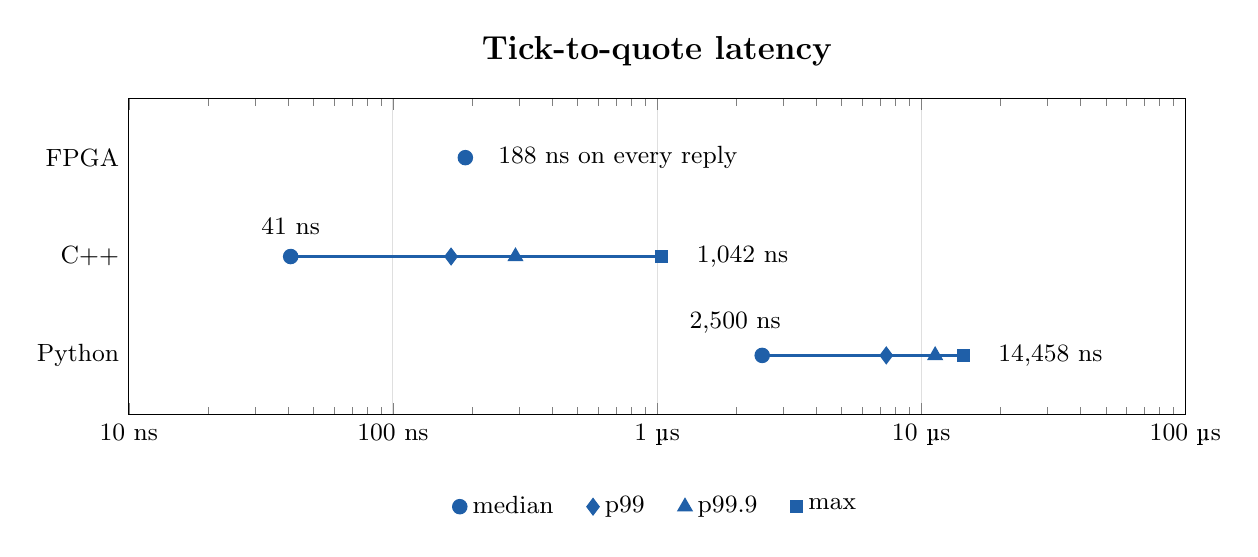
\begin{tikzpicture}
\begin{axis}[
  width=15cm, height=5.6cm,
  title={\textbf{Tick-to-quote latency}}, title style={font=\large, yshift=2pt},
  xmode=log, xmin=10, xmax=100000,
  ymin=0.4, ymax=3.6,
  ytick={1,2,3}, yticklabels={Python, C++, FPGA},
  xtick={10,100,1000,10000,100000},
  xticklabels={10 ns, 100 ns, 1 \textmu s, 10 \textmu s, 100 \textmu s},
  xmajorgrids, grid style={gray!25}, y tick style={draw=none},
  tick label style={font=\small},
  legend style={at={(0.5,-0.22)}, anchor=north, legend columns=4, draw=none, font=\small,
                /tikz/every even column/.append style={column sep=10pt}},
  clip=false,
]
\addplot[accent, thick, forget plot] coordinates {(41,2) (1042,2)};
\addplot[accent, thick, forget plot] coordinates {(2500,1) (14458,1)};
\addplot[only marks, mark=*, mark size=2.6pt, accent] coordinates {(188,3) (41,2) (2500,1)};
\addplot[only marks, mark=diamond*, mark size=3pt, accent] coordinates {(166,2) (7375,1)};
\addplot[only marks, mark=triangle*, mark size=3pt, accent] coordinates {(291,2) (11291,1)};
\addplot[only marks, mark=square*, mark size=2.2pt, accent] coordinates {(1042,2) (14458,1)};
\legend{median, p99, p99.9, max}
\node[anchor=west, font=\small] at (axis cs:230,3) {188 ns on every reply};
\node[anchor=south, font=\small] at (axis cs:41,2.12) {41 ns};
\node[anchor=west, font=\small] at (axis cs:1300,2) {1{,}042 ns};
\node[anchor=south east, font=\small] at (axis cs:3200,1.12) {2{,}500 ns};
\node[anchor=west, font=\small] at (axis cs:18000,1) {14{,}458 ns};
\end{axis}
\end{tikzpicture}
\end{document}
